\section{Exercícios}

Agora que tens todos os conceitos e exemplos expostos anteriormente até o
momento, chega a hora de resolver exercícios referentes aos conteúdos!

\begin{enumerate}
	\item A corrente através de um elemento é ilustrada na Figura~\ref{fig:fig5}. Determine a carga total que passa pelo elemento em:
	      (a) \( t = 1 \) s, (b) \( t = 3 \) s, (c) \( t = 5 \) s.

	      \begin{figure}[H]
		      \centering
		      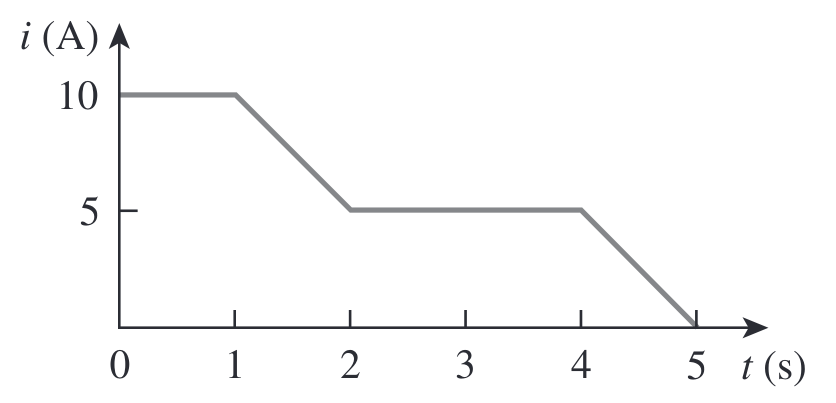
\includegraphics[height=0.15\textwidth]{./fig/fig5.png}
		      \caption{Forma de onda da corrente}
		      \label{fig:fig5}
	      \end{figure}

	      \[
		      i(t) =
		      \begin{cases}
			      10 \text{ A},              & 0 \leq t < 1 \text{ s}    \\
			      10 - 2.5(t - 1) \text{ A}, & 1 \leq t < 2 \text{ s}    \\
			      5 \text{ A},               & 2 \leq t < 4 \text{ s}    \\
			      5 - 2.5(t - 4) \text{ A},  & 4 \leq t \leq 5 \text{ s} \\
		      \end{cases}
	      \]

	      \begin{align*}
		      \text{(a)}\quad &
		      \begin{aligned}[t]
			      Q & = \int_{0}^{1} 10 \,dt = 10 \,\text{C}
		      \end{aligned}
		      \\
		      \text{(b)}\quad &
		      \begin{aligned}[t]
			      Q & = \int_{0}^{1} 10 \,dt + \int_{1}^{2} (10 - 2.5(t-1)) \,dt + \int_{2}^{3} 5 \,dt \\
			        & = 10 + 8.75 + 5                                                                  \\
			        & = 23.75 \,\text{C}
		      \end{aligned}
		      \\
		      \text{(c)}\quad &
		      \begin{aligned}[t]
			      Q & = \int_{0}^{1} 10 \,dt + \int_{1}^{2} (10 - 2.5(t-1)) \,dt     \\
			        & \quad + \int_{2}^{4} 5 \,dt + \int_{4}^{5} (5 - 2.5(t-4)) \,dt \\
			        & = 10 + 8.75 + 10 + 3.75                                        \\
			        & = 32.5 \,\text{C}
		      \end{aligned}
	      \end{align*}
	\item A carga que entra em determinado elemento é mostrada na
	      Figura~\ref{fig:fig6}. Determine a corrente em: (a) \( t = 1 \) ms, (b)
	      \( t = 6 \) ms, (c) \( t = 10 \) ms,
	      \begin{figure}[H]
		      \centering
		      \setlength{\fboxsep}{0pt}
		      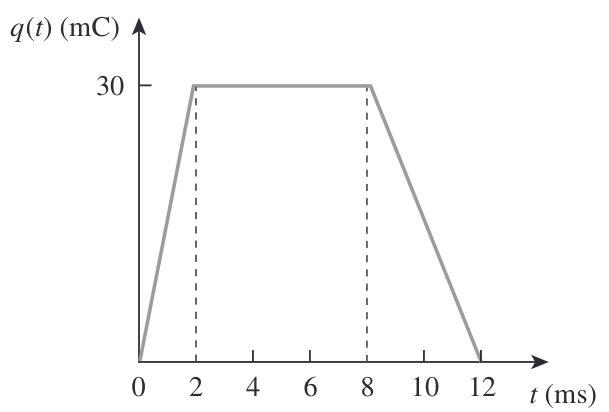
\includegraphics[height=0.2\textwidth]{./fig/fig6.png}
		      \caption{}
		      \label{fig:fig6}
	      \end{figure}
	      \begin{aligned}[t]
		      q(t) =
		      \begin{cases}
			      15t \, \text{mC},             & 0 \leq t < 2 \, \text{ms}      \\
			      30 \, \text{mC},              & 2 \leq t < 10 \, \text{ms}     \\
			      30 - 15(t - 10) \, \text{mC}, & 10 \leq t \leq 12 \, \text{ms} \\
		      \end{cases}
	      \end{aligned}
	      \vspace{6pt}
	      \begin{aligned}[t]
		      i(t) =
		      \begin{cases}
			      15 \, \text{mA},  & 0 < t < 2 \, \text{ms}   \\
			      0 \, \text{mA},   & 2 < t < 10 \, \text{ms}  \\
			      -15 \, \text{mA}, & 10 < t < 12 \, \text{ms} \\
		      \end{cases}
	      \end{aligned}
	      \vspace{6pt}
	      \begin{aligned}[t]
		      \text{(a)}\quad & i(1 \, \text{ms}) = 15 \, \text{mA}   \\
		      \text{(b)}\quad & i(6 \, \text{ms}) = 0 \, \text{mA}    \\
		      \text{(c)}\quad & i(10 \, \text{ms}) = -15 \, \text{mA} \\
	      \end{aligned}
	      \vspace{10pt}
	\item A corrente que fui por um ponto em um dispositivo é mostrada na
	      Figura~\ref{fig:fig7}. Calcule a carga total através do ponto.
	      \begin{figure}[H]
		      \centering
		      \setlength{\fboxsep}{0pt}
		      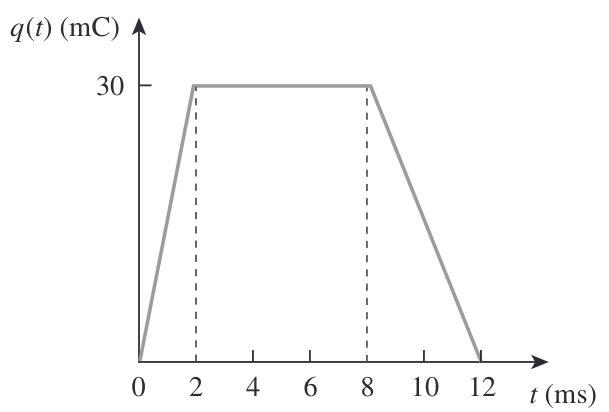
\includegraphics[height=0.15\textwidth]{./fig/fig7.png}
		      \caption{}
		      \label{fig:fig7}
	      \end{figure}
	      \begin{aligned}[t]
		      i(t) =
		      \begin{cases}
			      10t \, \text{mC}, & 0 \leq t < 1 \, \text{ms} \\
			      10 \, \text{mC},  & 1 \leq t < 2 \, \text{ms} \\
		      \end{cases}
	      \end{aligned}
	      \vspace{6pt}
	      \begin{aligned}[t]
		      Q & = \int_{0}^{1} 10t \, dt + \int_{1}^{2} 10 \, dt \\
		        & = 10 \int_{0}^{1} t \, dt + (20 - 10)            \\
		        & = 10 \frac{1}{2} \, dt + 10                      \\
		        & = 5 \, \text{mC} + 10 \, \text{mC}               \\
		        & = 15 \, \text{mC}                                \\
	      \end{aligned}
	      \newpage
	\item As Figuras~\ref{fig:fig8} e~\ref{fig:fig9} mostram a corrente e a tensão em um dispositivo.
	      \begin{enumerate}
		      \item Esboce o gráfico da potência liberada para o dispositivo para \( t > 0 \).

		            \begin{figure}[H]
			            \centering
			            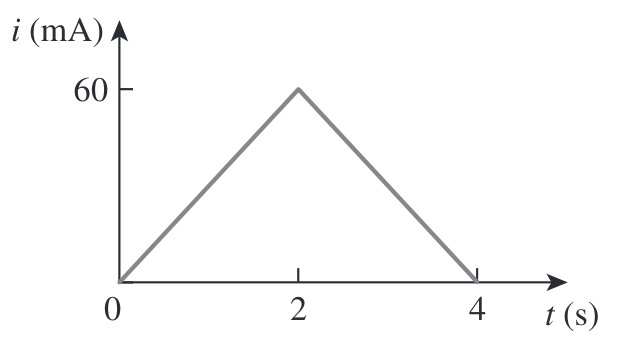
\includegraphics[height=0.15\textwidth]{./fig/fig8.png}
			            \caption{}
			            \label{fig:fig8}
		            \end{figure}
		            \begin{figure}[H]
			            \centering
			            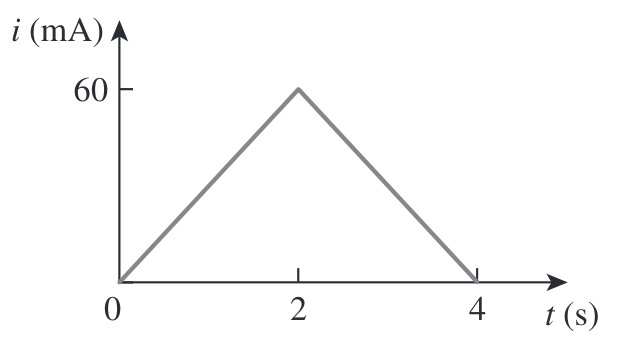
\includegraphics[height=0.15\textwidth]{./fig/fig9.png}
			            \caption{}
			            \label{fig:fig9}
		            \end{figure}

		            \begin{minipage}{\linewidth}
			            \begin{align*}
				            p(t)         & = v(t) \cdot i(t)                                                      \\
				            \text{Para } & 0 < t < 2 \text{ s:}                                                   \\
				            p(t)         & = 5 \, \text{V} \times 30t \, \text{mA} = 150t \, \text{mW}            \\
				                         & \text{\quad Potência positiva e linear (dispositivo absorve energia).} \\
				            \text{Para } & 2 \leq t \leq 4 \text{ s:}                                             \\
				            p(t)         & = -5 \, \text{V} \times (120 - 30t) \, \text{mA}                       \\
				                         & = -600 + 150t \, \text{mW}                                             \\
				                         & \text{\quad Potência negativa e linear (dispositivo fornece energia).} \\
			            \end{align*}
		            \end{minipage}

		            \begin{figure}[H]
			            \centering
			            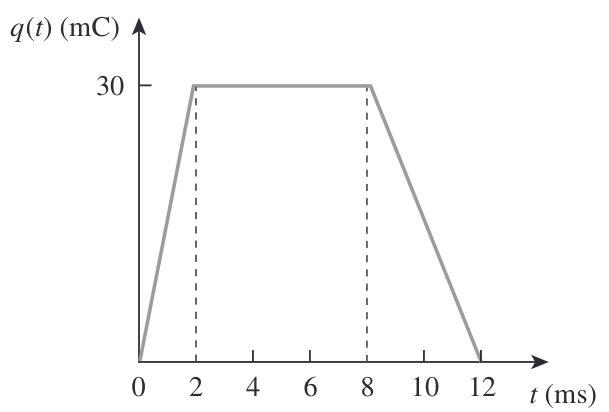
\includegraphics[height=0.25\textwidth]{./fig/fig10.png}
			            \caption{}
			            \label{fig:fig10}
		            \end{figure}

		      \item Determine a energia total absorvida pelo dispositivo para o período \( 0 < t < 4 \) s.

		            \begin{align*}
			            W & = \int_{0}^{4} p(t) \, dt                                    \\
			              & = \int_{0}^{2} 150t \, dt + \int_{2}^{4} (-600 + 150t) \, dt \\
			              & = \left[75t^2\right]_0^2 + \left[-600t + 75t^2\right]_2^4    \\
			              & = 300 \, \text{mJ} - 300 \, \text{mJ}                        \\
			              & = 0 \, \text{mJ}                                             \\
		            \end{align*}
	      \end{enumerate}
\end{enumerate}
